\documentclass[conference]{IEEEtran}

\usepackage{cite}
\usepackage{amsmath,amssymb}
\usepackage{array}
\usepackage{booktabs}
\usepackage{graphicx}
\usepackage{tabularx}
\usepackage{threeparttable}
\usepackage{url}
\usepackage{algorithm}
\usepackage{algorithmic}
\usepackage{tikz}
\usetikzlibrary{arrows.meta,calc,fit,positioning,shapes.geometric}

\graphicspath{{figures/}}
\tikzset{
  paperblock/.style={draw, rounded corners, align=center, fill=blue!5, minimum height=8mm, inner sep=4pt, font=\small},
  papersmall/.style={draw, rounded corners, align=center, fill=green!6, minimum height=7mm, inner sep=3pt, font=\scriptsize},
  papertensor/.style={draw, align=center, fill=orange!10, minimum height=8mm, inner sep=4pt, font=\small},
  paperarrow/.style={-{Latex[length=2mm]}, thick},
  paperfeedback/.style={-{Latex[length=2mm]}, thick, dashed}
}

\newcommand{\HybridArchitectureDiagram}{%
\resizebox{\textwidth}{!}{%
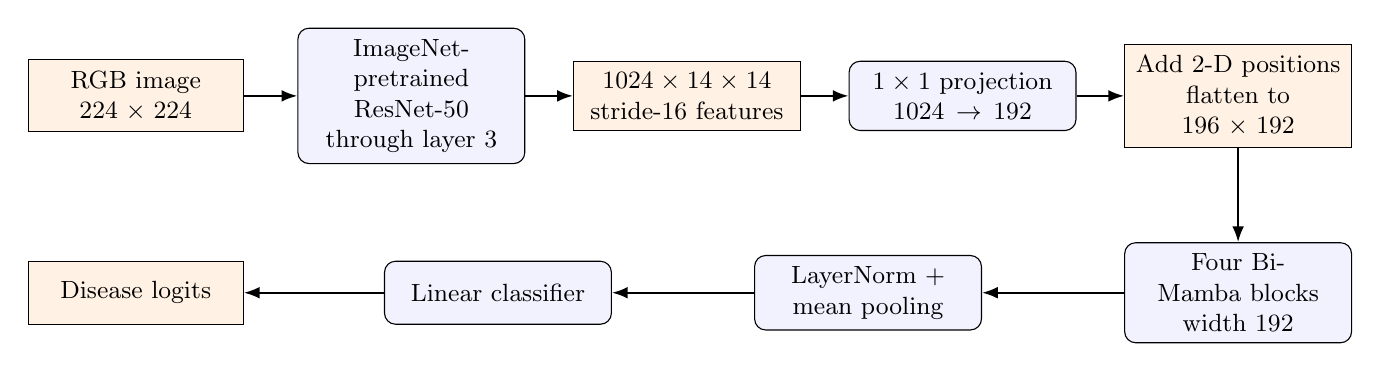
\begin{tikzpicture}[x=1cm,y=1cm]
  \node[papertensor,text width=2.45cm] (input) at (0,1.25) {RGB image\\$224\times224$};
  \node[paperblock,text width=2.6cm] (cnn) at (3.5,1.25) {ImageNet-pretrained\\ResNet-50 through layer 3};
  \node[papertensor,text width=2.6cm] (features) at (7.0,1.25) {$1024\times14\times14$\\stride-16 features};
  \node[paperblock,text width=2.6cm] (projection) at (10.5,1.25) {$1\times1$ projection\\$1024\rightarrow192$};
  \node[papertensor,text width=2.6cm] (tokens) at (14.0,1.25) {Add 2-D positions\\flatten to $196\times192$};
  \node[paperblock,text width=2.6cm] (mamba) at (14.0,-1.25) {Four Bi-Mamba blocks\\width 192};
  \node[paperblock,text width=2.6cm] (pool) at (9.3,-1.25) {LayerNorm +\\mean pooling};
  \node[paperblock,text width=2.6cm] (head) at (4.6,-1.25) {Linear classifier};
  \node[papertensor,text width=2.45cm] (output) at (0,-1.25) {Disease logits};
  \draw[paperarrow] (input) -- (cnn);
  \draw[paperarrow] (cnn) -- (features);
  \draw[paperarrow] (features) -- (projection);
  \draw[paperarrow] (projection) -- (tokens);
  \draw[paperarrow] (tokens.south) -- (mamba.north);
  \draw[paperarrow] (mamba.west) -- (pool.east);
  \draw[paperarrow] (pool.west) -- (head.east);
  \draw[paperarrow] (head.west) -- (output.east);
\end{tikzpicture}%
}%
}

\newcommand{\CNNTokenDiagram}{%
\resizebox{\textwidth}{!}{%
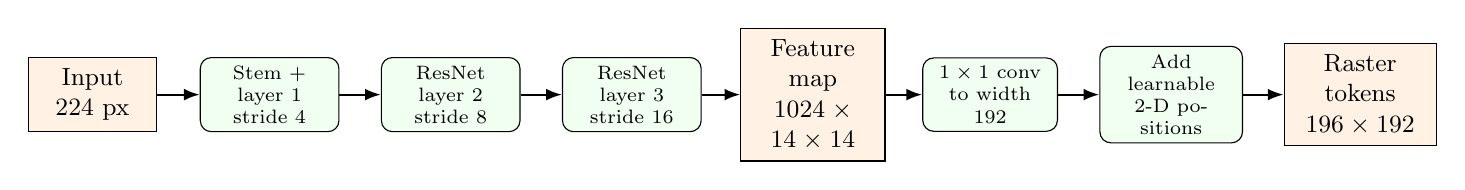
\begin{tikzpicture}[x=1cm,y=1cm]
  \node[papertensor,text width=1.35cm] (input) at (0,0) {Input\\224 px};
  \node[papersmall,text width=1.55cm] (stem) at (2.25,0) {Stem +\\layer 1\\stride 4};
  \node[papersmall,text width=1.55cm] (layer2) at (4.55,0) {ResNet\\layer 2\\stride 8};
  \node[papersmall,text width=1.55cm] (layer3) at (6.85,0) {ResNet\\layer 3\\stride 16};
  \node[papertensor,text width=1.55cm] (map) at (9.15,0) {Feature map\\$1024\times14\times14$};
  \node[papersmall,text width=1.5cm] (proj) at (11.4,0) {$1\times1$ conv\\to width 192};
  \node[papersmall,text width=1.6cm] (position) at (13.7,0) {Add learnable\\2-D positions};
  \node[papertensor,text width=1.65cm] (flatten) at (16.1,0) {Raster tokens\\$196\times192$};
  \foreach \a/\b in {input/stem,stem/layer2,layer2/layer3,layer3/map,map/proj,proj/position,position/flatten}
    \draw[paperarrow] (\a) -- (\b);
\end{tikzpicture}%
}%
}

\newcommand{\BiMambaDiagram}{%
\resizebox{\textwidth}{!}{%
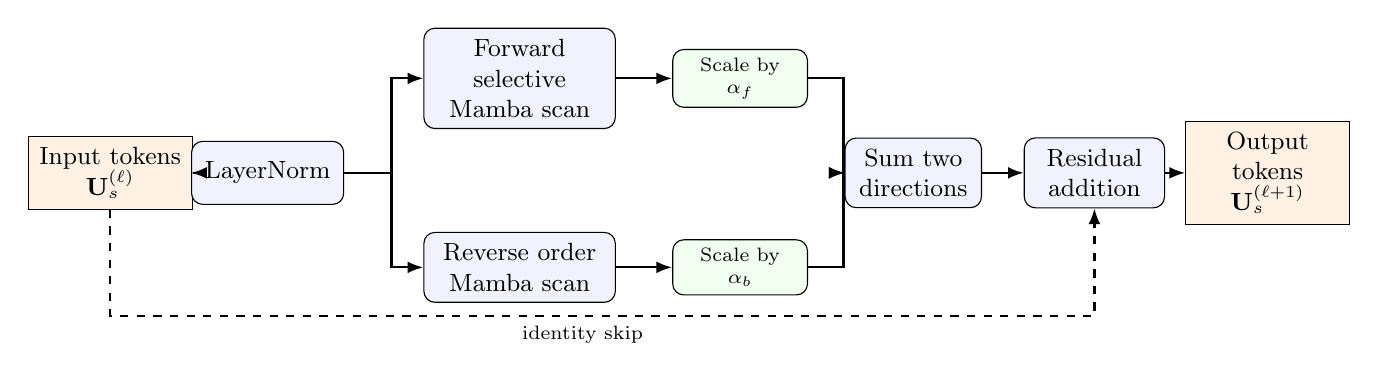
\begin{tikzpicture}[x=1cm,y=1cm]
  \node[papertensor,text width=1.8cm] (input) at (0,0) {Input tokens\\$\mathbf{U}_s^{(\ell)}$};
  \node[paperblock,text width=1.65cm] (norm) at (2.0,0) {LayerNorm};
  \node[paperblock,text width=2.15cm] (forward) at (5.2,1.2) {Forward selective\\Mamba scan};
  \node[paperblock,text width=2.15cm] (reverse) at (5.2,-1.2) {Reverse order\\Mamba scan};
  \node[papersmall,text width=1.5cm] (fweight) at (8.0,1.2) {Scale by\\$\alpha_f$};
  \node[papersmall,text width=1.5cm] (bweight) at (8.0,-1.2) {Scale by\\$\alpha_b$};
  \node[paperblock,text width=1.45cm] (sum) at (10.2,0) {Sum two\\directions};
  \node[paperblock,text width=1.5cm] (residual) at (12.5,0) {Residual\\addition};
  \node[papertensor,text width=1.8cm] (output) at (14.7,0) {Output tokens\\$\mathbf{U}_s^{(\ell+1)}$};
  \draw[paperarrow] (input) -- (norm);
  \draw[paperarrow] (norm.east) -- ++(0.6,0) |- (forward.west);
  \draw[paperarrow] (norm.east) -- ++(0.6,0) |- (reverse.west);
  \draw[paperarrow] (forward) -- (fweight);
  \draw[paperarrow] (reverse) -- (bweight);
  \draw[paperarrow] (fweight.east) -- ++(0.45,0) |- (sum.west);
  \draw[paperarrow] (bweight.east) -- ++(0.45,0) |- (sum.west);
  \draw[paperarrow] (sum) -- (residual);
  \draw[paperarrow] (residual) -- (output);
  \coordinate (skipStart) at ($(input.south)+(0,-1.35)$);
  \draw[paperfeedback] (input.south) -- (skipStart) -| (residual.south);
  \node[below,font=\scriptsize] at ($(skipStart)+(6.0,0)$) {identity skip};
\end{tikzpicture}%
}%
}

\newcommand{\SelfSupervisedDiagram}{%
\resizebox{\textwidth}{!}{%
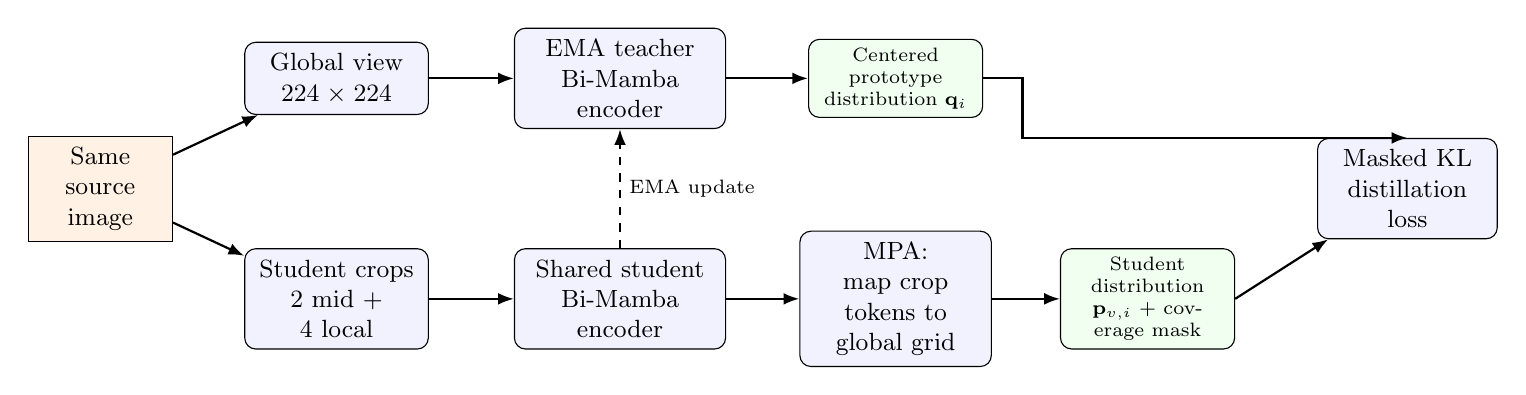
\begin{tikzpicture}[x=1cm,y=1cm]
  \node[papertensor,text width=1.55cm] (image) at (0,0) {Same source\\image};
  \node[paperblock,text width=2.05cm] (global) at (3.0,1.4) {Global view\\$224\times224$};
  \node[paperblock,text width=2.05cm] (crops) at (3.0,-1.4) {Student crops\\2 mid + 4 local};
  \node[paperblock,text width=2.4cm] (teacher) at (6.6,1.4) {EMA teacher\\Bi-Mamba encoder};
  \node[paperblock,text width=2.4cm] (student) at (6.6,-1.4) {Shared student\\Bi-Mamba encoder};
  \node[papersmall,text width=2.0cm] (teacherhead) at (10.1,1.4) {Centered prototype\\distribution $\mathbf{q}_i$};
  \node[paperblock,text width=2.15cm] (align) at (10.1,-1.4) {MPA: map crop\\tokens to global grid};
  \node[papersmall,text width=2.0cm] (studenthead) at (13.3,-1.4) {Student distribution\\$\mathbf{p}_{v,i}$ + coverage mask};
  \node[paperblock,text width=2.0cm] (loss) at (16.6,0) {Masked KL\\distillation loss};
  \draw[paperarrow] (image) -- (global);
  \draw[paperarrow] (image) -- (crops);
  \draw[paperarrow] (global) -- (teacher);
  \draw[paperarrow] (crops) -- (student);
  \draw[paperarrow] (teacher) -- (teacherhead);
  \draw[paperarrow] (student) -- (align);
  \draw[paperarrow] (align) -- (studenthead);
  \draw[paperarrow] (teacherhead.east) -- ++(0.5,0) |- (loss.north);
  \draw[paperarrow] (studenthead.east) -- (loss);
  \draw[paperfeedback] (student.north) -- node[midway,right=2pt,fill=white,inner sep=1pt,font=\scriptsize]{EMA update} (teacher.south);
\end{tikzpicture}%
}%
}

\newcommand{\ExperimentalWorkflowDiagram}{%
\resizebox{\textwidth}{!}{%
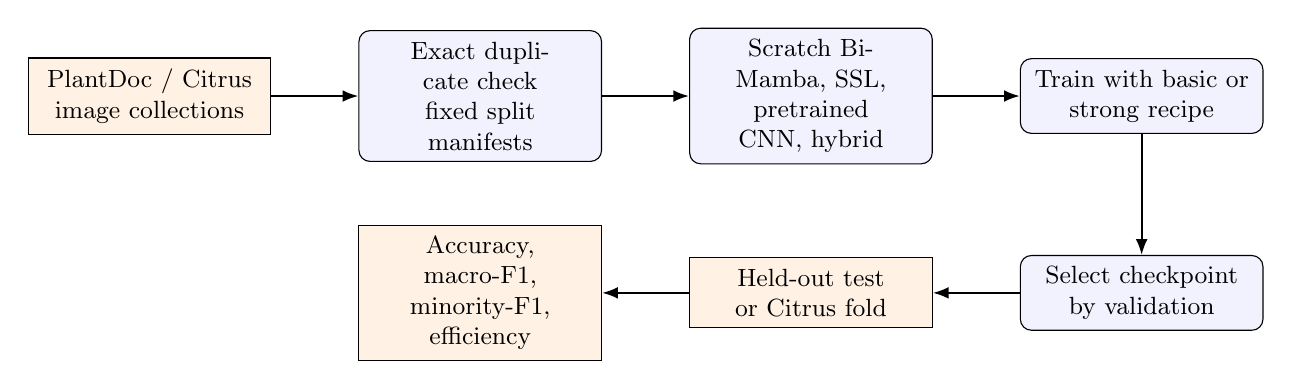
\begin{tikzpicture}[x=1cm,y=1cm]
  \node[papertensor,text width=2.8cm] (data) at (0,1.25) {PlantDoc / Citrus\\image collections};
  \node[paperblock,text width=2.8cm] (split) at (4.2,1.25) {Exact duplicate check\\fixed split manifests};
  \node[paperblock,text width=2.8cm] (models) at (8.4,1.25) {Scratch Bi-Mamba, SSL,\\pretrained CNN, hybrid};
  \node[paperblock,text width=2.8cm] (train) at (12.6,1.25) {Train with basic or\\strong recipe};
  \node[paperblock,text width=2.8cm] (select) at (12.6,-1.25) {Select checkpoint\\by validation};
  \node[papertensor,text width=2.8cm] (test) at (8.4,-1.25) {Held-out test\\or Citrus fold};
  \node[papertensor,text width=2.8cm] (metrics) at (4.2,-1.25) {Accuracy, macro-F1,\\minority-F1, efficiency};
  \draw[paperarrow] (data) -- (split);
  \draw[paperarrow] (split) -- (models);
  \draw[paperarrow] (models) -- (train);
  \draw[paperarrow] (train.south) -- (select.north);
  \draw[paperarrow] (select.west) -- (test.east);
  \draw[paperarrow] (test.west) -- (metrics.east);
\end{tikzpicture}%
}%
}

\begin{document}

\title{Pretrained CNN Features with Bidirectional Mamba for Plant Disease Recognition: A Reproduction and Controlled Study}

\author{\IEEEauthorblockN{Laxman \quad Sahil Singh}
\IEEEauthorblockA{Department of Computer Science and Engineering\\
Netaji Subhas University of Technology (NSUT), New Delhi, India\\
Project Supervisor: Assistant Professor Ankush Jain}}

\maketitle

\begin{abstract}
This study examines whether pretrained visual representations and bidirectional state-space blocks improve plant-disease recognition under small-data conditions. We reproduce a supervised Bi-Mamba baseline and a reduced-compute, self-supervised PSMamba-style pretraining pipeline, then compare them with ImageNet-pretrained CNN references and a hybrid ResNet--Bi-Mamba model on PlantDoc and a five-class Citrus image collection. On the supplied PlantDoc split, the from-scratch Bi-Mamba reaches 33.73\% after 150 epochs, while the hybrid with a stronger regularization recipe reaches 74.60\%~$\pm$~0.69\% across three runs, with macro-F1 73.56\%~$\pm$~0.83\% and minority-class F1 62.64\%~$\pm$~3.41\%. A matched-recipe ResNet-50 reaches 71.43\%~$\pm$~3.39\%; the small-run comparison does not establish that Mamba blocks cause the observed difference. On Citrus, the from-scratch baseline obtains 90.61\%~$\pm$~2.24\% across five folds, while pretrained models cluster near 95\%; ConvNeXt-Tiny at 224 pixels obtains 95.72\%~$\pm$~0.70\%. Self-supervised initialization does not improve on the longer-trained from-scratch baseline in the available PlantDoc comparison. The reported PSMamba PlantDoc score is not reproduced, and the Citrus comparison is not like-for-like because the dataset copy and split differ. Overall, the evidence supports transfer from pretrained visual features, but is insufficient to isolate an additional benefit from the Mamba blocks or to claim general superiority.
\end{abstract}

\begin{IEEEkeywords}
Plant disease recognition, computer vision, state-space models, Mamba, self-supervised learning, transfer learning, class imbalance.
\end{IEEEkeywords}

\section{Introduction}
Visual disease recognition is challenging outside controlled image settings: leaf appearance varies with illumination, viewpoint, background, cultivar, disease stage, and image quality. These factors are especially consequential when datasets are small and disease classes are imbalanced. CNN-based plant-disease classifiers have demonstrated the potential of learned visual features, while also highlighting the distinction between controlled imagery and field images \cite{mohanty2016plantdisease,singh2020plantdoc}.

Selective state-space models provide a sequence-processing alternative to attention, with input-dependent state transitions and linear scaling in sequence length under the selective-scan formulation \cite{gu2024mamba}. Vision Mamba applies bidirectional state-space processing to image tokens \cite{zhu2024visionmamba}. PSMamba combines a bidirectional Mamba encoder with progressive, multi-scale self-supervised patch alignment for plant-disease recognition \cite{almamun2026psmamba}. Its reported PlantDoc and Citrus accuracies, as recorded in the supplied project report, are 95.64\% and 92.26\%, respectively. Our experiments do not reproduce the PlantDoc result; direct numerical comparison is also limited by dataset-copy and split differences.

We therefore frame this work as a reproduction and controlled experimental study, not as a state-of-the-art claim. We evaluate a from-scratch Bi-Mamba, a PSMamba-style self-supervised initialization, standard ImageNet-pretrained references, and a hybrid that uses a pretrained ResNet-50 feature extractor followed by randomly initialized Bi-Mamba blocks. The main PlantDoc result is 74.60\%~$\pm$~0.69\% for the hybrid under a stronger training recipe, compared with 33.73\% for the 150-epoch from-scratch Bi-Mamba. A ResNet-50 control under the same strong recipe reaches 71.43\%~$\pm$~3.39\%. Because the two multi-run samples are small and variable, this difference is suggestive rather than conclusive evidence for the sequence blocks.

The contributions are: (1) an explicit reproduction protocol with dataset-version and evaluation caveats; (2) controlled comparisons that distinguish scratch training, self-supervised initialization, pretrained CNN features, and training-recipe changes; (3) macro-F1 and minority-class analyses alongside accuracy; and (4) an efficiency profile that reports the limitations of the pure-PyTorch Mamba implementation rather than treating parameter count as a proxy for speed.

\section{Related Work}
\subsection{Plant-Disease Recognition}
Mohanty \textit{et al.} studied deep CNN classification of plant diseases in the PlantVillage setting \cite{mohanty2016plantdisease}. PlantDoc extends the problem to images with more varied, in-the-wild conditions and supplies a visual detection and classification dataset \cite{singh2020plantdoc}. These datasets differ substantially in scale and acquisition conditions; results on one should not be assumed to transfer to the other.

\subsection{Convolutional and Pretrained Visual Features}
Residual networks provide a deep convolutional feature hierarchy and are a common transfer-learning baseline \cite{he2016resnet}. ImageNet pretraining supplies broad visual representations learned from a large labeled image corpus \cite{deng2009imagenet}. ConvNeXt revisits convolutional design using modern training and architectural choices \cite{liu2022convnext}, while Swin Transformer uses hierarchical shifted-window attention \cite{liu2021swin}. These architectures are included as references, not as directly controlled tests of a single architectural factor.

\subsection{State-Space Vision Models}
Mamba introduces selective state-space layers for sequence modeling \cite{gu2024mamba}; Vision Mamba adapts bidirectional state-space processing to image patches \cite{zhu2024visionmamba}. PSMamba uses multi-scale teacher--student learning to align crop-level features with a global token grid \cite{almamun2026psmamba}. Our Bi-Mamba implementation follows the reported bidirectional encoder pattern, but uses a pure-PyTorch scan in the experimental environment. Consequently, its measured throughput is an implementation-specific property and should not be interpreted as the hardware efficiency of a fused selective-scan implementation.

\subsection{Self-Supervision and Regularization}
DINO established a teacher--student self-distillation approach with an exponential-moving-average teacher and centered teacher outputs \cite{caron2021dino}. The PSMamba-style experiment here follows the multi-scale alignment objective but changes the projection head after an implementation-level collapse was observed. Mixup, CutMix, and RandAugment are used as components of the stronger supervised recipe \cite{zhang2018mixup,yun2019cutmix,cubuk2020randaugment}. Because these components are applied together, this study cannot attribute gains to any one augmentation or to model EMA individually. AdamW is used for optimization \cite{loshchilov2019adamw}.

\section{Dataset and Leakage-Aware Preprocessing}
\subsection{Dataset Sources and Composition}
PlantDoc is a field-image dataset introduced for visual plant-disease detection \cite{singh2020plantdoc}. The supplied experiment uses a Kaggle copy with 2,670 images in its training folder and 252 in its test folder, giving 2,922 images before duplicate removal. The original dataset is reported to contain 2,598 images; therefore, this experiment does not use an identical dataset copy. After removal of byte-identical files across splits (five training images and one validation image), the fixed partition contains 2,131 training, 533 validation, and 252 test images. The training set has 28 classes; one class is absent from the test set, which contains 27 classes.

The Citrus image collection is based on a Kaggle copy associated with the citrus-disease images described by Rauf \textit{et al.} \cite{rauf2019citrus}. It contains 607 images in five classes, rather than the 609 reported for the source dataset: Black spot (169), Canker (163), Greening (204), Healthy (58), and Melanose (13). Since this supplied copy has no predefined split, we use stratified five-fold cross-validation with seed 42. Each fold reserves 12.5\% of its training portion for validation and uses the remaining fold as test data (approximately 121 test images per fold). Table~\ref{tab:datasets} summarizes the experimental partitions. Figure~\ref{fig:workflow} shows the common evaluation workflow.

The exact Kaggle dataset copies used for this study are:
\begin{itemize}
    \item PlantDoc: \url{https://www.kaggle.com/datasets/nirmalsankalana/plantdoc-dataset}
    \item Citrus: \url{https://www.kaggle.com/datasets/myprojectdictionary/citrus-leaf-disease-image}
\end{itemize}

\newcommand{\DatasetTable}{%
\begin{table}[t]
\caption{Dataset Composition and Evaluation Partitions}
\label{tab:datasets}
\centering
\footnotesize
\begin{tabularx}{\columnwidth}{@{}lXX@{}}
\toprule
Dataset & Composition & Partition used in this study \\
\midrule
PlantDoc copy & 2,670 train-folder images; 252 test-folder images; 28 train classes & 2,131 train / 533 validation / 252 test; 27 classes present in test \\
Citrus copy & 607 images: Black spot 169; Canker 163; Greening 204; Healthy 58; Melanose 13 & Stratified five-fold CV; about 121 test images per fold; 12.5\% of each training portion held for validation \\
\bottomrule
\end{tabularx}
\end{table}%
}

\newcommand{\PlantDocResultsTable}{%
\begin{table*}[t]
\caption{PlantDoc Results on the Supplied Fixed Test Split}
\label{tab:plantdoc-results}
\centering
\begin{threeparttable}
\scriptsize
\setlength{\tabcolsep}{3.2pt}
\begin{tabularx}{\textwidth}{@{}l l X c r r r@{}}
\toprule
Model & Initialization & Training setup & Runs & Accuracy (\%) & Macro-F1 (\%) & Minority F1 (\%) \\
\midrule
Bi-Mamba & Scratch & Basic, 50 epochs & 1 & 28.97 & 22.86 & 3.03 \\
Bi-Mamba & Scratch & Basic, 150 epochs & 1 & 33.73 & 30.92 & 17.53 \\
Bi-Mamba + SSL & Scratch + SSL & SSL 50 ep.; fine-tune 50 ep. & 1 & 33.33 & 29.73 & 14.94 \\
Bi-Mamba + SSL & Scratch + SSL & SSL 50 ep.; fine-tune 150 ep. & 1 & 33.33 & 30.08 & 20.69 \\
ResNet-50 & ImageNet & Basic, 20 epochs & 3 & $69.71\pm1.79$ & $69.09\pm1.20$ & $59.25\pm3.01$ \\
CNN--Bi-Mamba & ImageNet CNN & Basic, 30 epochs & 4$^{\dagger}$ & $68.95\pm1.56$ & $68.04\pm1.42$ & $57.57\pm7.02$ \\
ResNet-50 & ImageNet & Strong, 45 epochs & 3 & $71.43\pm3.39$ & $71.17\pm3.20$ & $63.04\pm5.69$ \\
ConvNeXt-Tiny & ImageNet & Strong, 45 epochs & 1 & 73.41 & 72.62 & 64.95 \\
Swin-T & ImageNet & Strong, 45 epochs & 1 & 71.03 & 70.00 & 56.14 \\
CNN--Bi-Mamba & ImageNet CNN & Strong, 45 epochs & 3 & $74.60\pm0.69$ & $73.56\pm0.83$ & $62.64\pm3.41$ \\
\midrule
PSMamba (published) & -- & Reported score; different protocol & -- & 95.64 & -- & -- \\
\bottomrule
\end{tabularx}
\begin{tablenotes}[flushleft]
\footnotesize
\item Except for the published PSMamba score, values are test-set percentages. For multi-run rows, mean~$\pm$~sample standard deviation is across independent runs. Single-run entries are shown without a dispersion estimate. The published score is not a result from our split and is included only for context. Minority F1 is averaged over the rarest quartile of training classes present in the test set.
\item[$\dagger$] The supplied report gives a four-run aggregate, but only three PlantDoc basic-hybrid run records appear in the bundled CSV files. The reported aggregate is retained and requires author verification against the missing run log.
\end{tablenotes}
\end{threeparttable}
\end{table*}%
}

\newcommand{\CitrusResultsTable}{%
\begin{table*}[t]
\caption{Citrus Results: Five-Fold Stratified Evaluation}
\label{tab:citrus-results}
\centering
\begin{threeparttable}
\scriptsize
\setlength{\tabcolsep}{3.2pt}
\begin{tabularx}{\textwidth}{@{}l l X r r r@{}}
\toprule
Model & Resolution & Aggregation / recipe & Accuracy (\%) & Macro-F1 (\%) & Minority F1 (\%) \\
\midrule
Bi-Mamba, scratch & 224 & 5 folds, 1 seed & $90.61\pm2.24$ & $88.50\pm4.20$ & $85.48\pm10.78$ \\
ResNet-50, pretrained & 224 & 5 folds, 1 seed & $93.90\pm1.27$ & $95.52\pm0.87$ & $98.61\pm2.05$ \\
CNN--Bi-Mamba, basic (A) & 224 & 5 folds, 1 seed & $95.38\pm1.26$ & $95.31\pm3.41$ & $95.28\pm6.94$ \\
CNN--Bi-Mamba, basic (B) & 224 & 5 folds, 1 seed$^{\dagger}$ & $94.89\pm2.06$ & 94.84 & -- \\
CNN--Bi-Mamba, strong & 224 & 5 folds, 1 seed & $95.22\pm1.08$ & $95.19\pm3.09$ & -- \\
ConvNeXt-Tiny, strong & 224 & 5 folds, 1 seed & $95.72\pm0.70$ & $96.90\pm0.47$ & -- \\
ConvNeXt-Tiny, strong & 320 & 3 seeds $\times$ 5 folds$^{\ddagger}$ & $95.06\pm1.03$ & $96.14\pm1.04$ & -- \\
\midrule
PSMamba (published) & -- & Reported score; different protocol & 92.26 & -- & -- \\
\bottomrule
\end{tabularx}
\begin{tablenotes}[flushleft]
\footnotesize
\item For five-fold single-seed rows, mean~$\pm$~sample standard deviation is across folds. For ConvNeXt-Tiny at 320 pixels, each seed is first averaged across five folds; the table gives the mean~$\pm$~sample standard deviation of the three seed-level means. Macro-F1 and minority F1 dispersions for rows with available fold logs are computed from those logs. Dashes indicate metrics not available in the supplied records.
\item[$\dagger$] The report lists a second basic-hybrid five-fold run, but its fold-level CSV entries are absent from the project bundle; author verification is required.
\item[$\ddagger$] The three ConvNeXt-Tiny 320-pixel seed-level accuracy means are 96.21\%, 94.24\%, and 94.73\%. The reported aggregate is calculated from the bundled fold-level CSV files.
\item The published PSMamba Citrus score is not evaluated on these folds and is shown only as context.
\end{tablenotes}
\end{threeparttable}
\end{table*}%
}

\newcommand{\EfficiencyTable}{%
\begin{table*}[t]
\caption{Tesla T4 Efficiency Profile (FP16; Randomly Initialized Models)}
\label{tab:efficiency}
\centering
\begin{threeparttable}
\footnotesize
\setlength{\tabcolsep}{5pt}
\begin{tabularx}{\textwidth}{@{}X r r r r r r@{}}
\toprule
Model & Parameters (M) & GMACs$^{*}$ & Inference (img/s) & Inference memory (GB) & Training (img/s) & Training memory (GB) \\
\midrule
Bi-Mamba, scratch & 4.22 & 0.81 & 75.6 & 1.07 & 25.6 & 5.94 \\
CNN--Bi-Mamba & 10.80 & 3.71 & 131.6 & 1.12 & 43.6 & 4.05 \\
ResNet-50 & 23.57 & 4.09 & 837.1 & 0.36 & 229.5 & 1.19 \\
ConvNeXt-Tiny & 27.84 & 4.45 & 709.3 & 0.44 & 169.9 & 1.55 \\
Swin-T & 27.54 & 4.49 & 503.0 & 0.57 & 153.0 & 1.69 \\
\bottomrule
\end{tabularx}
\begin{tablenotes}[flushleft]
\footnotesize
\item Profiled on one NVIDIA Tesla T4 using FP16, batch size 32 for inference and 16 for training. The source report describes random initialization for this profile. Throughput is specific to the project implementation; the Mamba scan uses a pure-PyTorch path.
\item[$^{*}$] Approximate GMAC count includes convolutions and matrix multiplications but undercounts or omits the sequential state-space scan.
\end{tablenotes}
\end{threeparttable}
\end{table*}%
}

\newcommand{\ControlledTable}{%
\begin{table*}[t]
\caption{Selected Controlled Comparisons and Interpretation}
\label{tab:controlled}
\centering
\footnotesize
\begin{tabularx}{\textwidth}{@{}X l r X@{}}
\toprule
Comparison & Dataset & Difference (pp) & Interpretation \\
\midrule
Bi-Mamba, 50 to 150 epochs & PlantDoc & $+4.76$ & Longer scratch training improves the baseline; 50 epochs is not a sufficient convergence control. \\
Scratch Bi-Mamba 150 ep. vs. SSL + fine-tune 150 ep. & PlantDoc & $-0.40$ & No measurable gain from the implemented self-supervised initialization at the matched fine-tuning budget. \\
Hybrid basic vs. strong recipe & PlantDoc & $+5.65$ & The combined stronger recipe improves the reported hybrid mean; individual components are not isolated. \\
ResNet-50 strong vs. hybrid strong & PlantDoc & $+3.17$ & Small three-run means favor the hybrid, but do not establish a reliable Mamba contribution. \\
Hybrid basic (A) vs. scratch Bi-Mamba & Citrus & $+4.78$ & Pretrained CNN features coincide with a higher five-fold mean; not a same-architecture causal contrast. \\
Hybrid basic (A) vs. hybrid strong & Citrus & $-0.16$ & The strong recipe does not provide a consistent additional improvement in this run set. \\
ConvNeXt-Tiny 224 vs. 320, three-seed mean & Citrus & $-0.66$ & Higher resolution does not improve the three-seed average; the 96.21\% single-seed result is not representative. \\
ConvNeXt-Tiny 320, flip TTA vs. no TTA & Citrus & $+0.11$ & Mean change across seed-level fold means is small and inconsistent by fold. \\
\bottomrule
\end{tabularx}
\end{table*}%
}
\DatasetTable

The Kaggle URLs above identify the exact mirrors used for this study, but exact dataset version identifiers, access dates, and license details should still be recorded in the final reproducibility package. The canonical PlantDoc and Citrus papers cited above describe the source datasets, not necessarily every detail of these exact mirrors.

\subsection{Splits, Preprocessing, and Leakage Controls}
The fixed PlantDoc split and stratified Citrus folds are established before model training. An exact byte-level duplicate check is applied across split boundaries; the report records five duplicate training files and one validation file removed for PlantDoc. RGB images are used throughout. Training augmentations depend on the basic or strong recipe, while evaluation images are resized to the selected model resolution and normalized using ImageNet channel statistics. Checkpoints are selected using validation data, and the held-out test partition is evaluated only with the selected checkpoint. PlantDoc uses one fixed test split; Citrus metrics are summarized across five folds. Reported mean~$\pm$~standard deviation therefore refers to independent seeds for PlantDoc multi-run rows and to folds for Citrus rows, except where the table explicitly identifies variation across seed-level five-fold means.

This protocol reduces leakage from exact duplicate files and from using evaluation partitions for gradient updates, but it does not establish that every form of leakage is absent. No perceptual near-duplicate screening or source-plant grouping is documented, so visually similar images may remain across partitions. Macro-F1 averages per-class F1 over classes present in the evaluated test split. Minority-class F1 averages the F1 of classes in the rarest quartile by training-set frequency among classes present in the test set; consequently, the absent PlantDoc test class is excluded, and Citrus minority-class F1 is sensitive to the few Melanose examples in each fold.

\section{Problem Formulation and Research Objectives}
Let $\mathcal{D}=\{(x_i,y_i)\}_{i=1}^{N}$ denote a labeled image collection with $C$ disease classes. We study a multi-class classifier $f_{\theta}:\mathcal{X}\rightarrow\mathbb{R}^{C}$ that maps an RGB leaf image to class logits. The experimental question is not whether a model can attain a particular headline score on a different dataset copy, but how the measured performance changes under the supplied split when the representation, pretraining, and training recipe are varied.

The study addresses four questions:
\begin{enumerate}
    \item How does a supervised Bi-Mamba trained from scratch compare with pretrained CNN and hybrid alternatives on PlantDoc and Citrus?
    \item Does the available PSMamba-style self-supervised initialization improve the supervised Bi-Mamba result under the evaluated training budgets?
    \item Do stronger regularization and augmentation strategies change performance, especially on the small PlantDoc split?
    \item Do the available controls isolate an independent benefit from adding Bi-Mamba blocks after pretrained CNN features?
\end{enumerate}

The study is exploratory. PlantDoc has one fixed held-out test split and Citrus has five stratified folds; these evaluation units are not interchangeable. We report them separately and avoid significance claims unsupported by the run counts.

\section{Methodology}
\subsection{PSMamba and Bidirectional Mamba Formulation}
Following the notation of PSMamba, let $x$ denote an image and let $s\in\{G,M,L\}$ index its global, mid-scale, and local views, generated by crop operators $\phi_s$. The original method uses view sizes $224\times224$, $160\times160$, and $96\times96$ pixels and a patch stride of 32, giving token grids of $7\times7$, $5\times5$, and $3\times3$, respectively \cite{almamun2026psmamba}. Our reproduction retains these view sizes but uses the stride-16 patch embedding of the implemented Bi-Mamba encoder, giving grids of $14\times14$, $10\times10$, and $6\times6$. We state the distinction because the reproduction is not an exact architectural replication of the published tokenization.

Let $\Lambda_s=\{v_j\}_{j=1}^{N_s}$ denote the two-dimensional token grid for view $s$. A fixed rasterization $\pi_s:\Lambda_s\rightarrow\{1,\ldots,N_s\}$ maps each grid location to the one-dimensional scan order, while $\pi_s^{-1}$ retains its spatial coordinates for alignment. The encoder maps a view to contextualized features
\begin{equation}
    \mathbf{Z}_s=f_{\theta}(\phi_s(x))\in\mathbb{R}^{N_s\times d}.
    \label{eq:view-tokens}
\end{equation}

For a continuous-time state-space model, the latent state and output satisfy
\begin{align}
    \dot{\mathbf{h}}(t) &= \mathbf{A}\mathbf{h}(t)+\mathbf{B}\mathbf{u}(t),\\
    \mathbf{z}(t) &= \mathbf{C}\mathbf{h}(t)+\mathbf{D}\mathbf{u}(t).
    \label{eq:ssm-continuous}
\end{align}
Under zero-order-hold discretization with step size $\Delta$, the state update is
\begin{equation}
    \bar{\mathbf{A}}=\exp(\Delta\mathbf{A}),\qquad
    \bar{\mathbf{B}}=\int_{0}^{\Delta}\exp(\tau\mathbf{A})\mathbf{B}\,d\tau.
    \label{eq:ssm-discretization}
\end{equation}
In a selective Mamba layer, the discretized parameters depend on the current input. For layer $\ell$, this recurrence can be written
\begin{align}
    \mathbf{h}^{(\ell)}_{t+1} &= \bar{\mathbf{A}}^{(\ell)}_t\mathbf{h}^{(\ell)}_t+\bar{\mathbf{B}}^{(\ell)}_t\mathbf{u}^{(\ell)}_t,\\
    \mathbf{z}^{(\ell)}_t &= \mathbf{C}^{(\ell)}_t\mathbf{h}^{(\ell)}_t+\mathbf{D}^{(\ell)}\mathbf{u}^{(\ell)}_t,
    \label{eq:ssm-selective}
\end{align}
where $t$ indexes the rasterized sequence. The source paper denotes bidirectional fusion as $\mathbf{z}_{s,t}^{(\ell)}=\mathbf{W}^{(\ell)}_f\overrightarrow{\mathbf{z}}_{s,t}^{(\ell)}+\mathbf{W}^{(\ell)}_b\overleftarrow{\mathbf{z}}_{s,t}^{(\ell)}$. Our implementation instead uses learnable scalar fusion coefficients and a residual connection. To capture context in both scan directions, define
\begin{align}
    \overrightarrow{\mathbf{Z}}_s^{(\ell)} &= \mathcal{M}^{(\ell)}_f\!\left(\widetilde{\mathbf{U}}_s^{(\ell)}\right),\\
    \overleftarrow{\mathbf{Z}}_s^{(\ell)} &= \operatorname{rev}\!\left[\mathcal{M}^{(\ell)}_b\!\left(\operatorname{rev}(\widetilde{\mathbf{U}}_s^{(\ell)})\right)\right],\\
    \mathbf{U}_s^{(\ell+1)} &= \mathbf{U}_s^{(\ell)}+\alpha_f\overrightarrow{\mathbf{Z}}_s^{(\ell)}+\alpha_b\overleftarrow{\mathbf{Z}}_s^{(\ell)},
    \label{eq:bimamba}
\end{align}
where $\widetilde{\mathbf{U}}_s^{(\ell)}=\operatorname{LN}(\mathbf{U}_s^{(\ell)})$, $\mathbf{U}_s^{(0)}$ is the input token sequence, and $\alpha_f$ and $\alpha_b$ are the learnable directional fusion scalars, initialized to 0.5 in our implementation. Equation~\eqref{eq:bimamba} makes explicit the forward and reversed scans, their alignment back to the original token order, and the residual path used by our block; Fig.~\ref{fig:bimamba-block} depicts the corresponding block.

\subsection{Bi-Mamba Supervised Baseline}
The scratch baseline embeds non-overlapping $16\times16$ image patches using a convolution with stride 16. The embedding width is 192, followed by a learnable two-dimensional positional embedding, eight Bi-Mamba blocks, layer normalization, global mean pooling, and a linear classifier. The encoder has approximately 4.22 million parameters. The Mamba state size is 16, the local convolution width is 4, and the expansion factor is 2. The implementation uses \texttt{mambapy} without the official fused CUDA kernels.

For an image batch $\mathbf{I}\in\mathbb{R}^{B\times3\times H\times W}$, the scratch model's initial patch tokens are
\begin{equation}
    \begin{aligned}
    \mathbf{U}^{(0)} &= \operatorname{Flatten}\!\left(\operatorname{Conv}_{16\times16,\,s=16}(\mathbf{I})+\mathbf{P}_{H/16\times W/16}\right),\\
    \mathbf{U}^{(0)} &\in\mathbb{R}^{B\times(HW/256)\times192}.
    \end{aligned}
    \label{eq:patch-tokens}
\end{equation}
Here, $\mathbf{P}$ is the learned positional grid, resized bicubically when the input resolution changes. The resulting tokens are contextualized by the Bi-Mamba layers in \eqref{eq:bimamba}.

\subsection{Critical Analysis of Baseline Methodology}
The from-scratch Bi-Mamba is a useful reference for measuring performance without ImageNet visual features, but it is not a capacity- or protocol-matched control for every pretrained model. Its single patch-embedding convolution and rasterized sequence provide less explicit local two-dimensional structure than a CNN, while its 4.22-million-parameter encoder is trained only on the supplied disease images. The low PlantDoc accuracy (33.73\%) and minority-class F1 (17.53\%) are consistent with difficulty learning transferable features and representing rare classes from this small, imbalanced training set; these results alone do not identify the cause.

The baseline's bidirectional scans provide context from both sequence directions, but rasterization still imposes an arbitrary one-dimensional ordering on a two-dimensional leaf. In addition, global mean pooling weights all final tokens uniformly and may dilute evidence from small lesions. These are architectural considerations, not experimentally isolated explanations for the measured errors. The baseline also uses a pure-PyTorch selective scan, so its throughput is implementation-dependent. Finally, the 50- and 150-epoch baseline runs show that training duration changes the result; comparisons against models with pretrained initialization, different optimizers, or stronger augmentation should therefore be interpreted as system-level comparisons rather than clean estimates of a single architectural effect.

\subsection{Self-Supervised Teacher--Student Reproduction}
The PSMamba-style pretraining uses one global teacher view and shared student weights for the mid and local crops. The original paper samples two global, six mid, and six local views; our compute-limited reproduction uses one global, two mid, and four local views per image. The teacher is an exponential-moving-average copy of the student encoder and head. In the supplied report, its momentum increases from 0.996 toward 0.999; teacher logits are centered with momentum 0.9. The report specifies 50 pretraining epochs, batch size 8, AdamW learning rate 1e-4, and weight decay 0.05. Student and teacher encoders use the scratch Bi-Mamba architecture. In the notation of \eqref{eq:view-tokens}, the teacher and student features are
\begin{equation}
    \mathbf{Z}^{t}_G=f_{\bar{\theta}}(\phi_G(x)),\qquad
    \mathbf{Z}_v=f_{\theta}(\phi_v(x)),\quad v\in\{M,L\}.
    \label{eq:teacher-features}
\end{equation}

Let $\bar{\theta}$ and $\theta$ denote teacher and student parameters, respectively. The teacher parameters and centered-logit vector are updated by exponential averages,
\begin{align}
    \bar{\theta}_{r+1} &\leftarrow \mu_r\bar{\theta}_{r}+(1-\mu_r)\theta_r,\\
    \mathbf{c}_{r+1} &\leftarrow \rho\mathbf{c}_{r}+(1-\rho)\frac{1}{BN_G}\sum_{b=1}^{B}\sum_{i=1}^{N_G}\boldsymbol{\ell}^{t}_{G,b,i},
    \label{eq:teacher-ema}
\end{align}
where $r$ indexes optimization steps, $\mu_r$ increases from 0.996 toward 0.999, $\rho=0.9$, and $N_G=196$ is the reproduction's global-grid token count. Let $H_{\bar{\theta}}$ and $H_{\theta}$ denote the teacher and student prototype heads. For global teacher features $\mathbf{Z}^{t}_G$ and the MPA-aligned student features $\widetilde{\mathbf{Z}}_v$, the logits and output distributions at global-grid cell $i$ are
\begin{align}
    \boldsymbol{\ell}^{t}_{G,i} &= H_{\bar{\theta}}\mathbf{Z}^{t}_G(i),\qquad
    \boldsymbol{\ell}^{s}_{v,i} = H_{\theta}\widetilde{\mathbf{Z}}_v(i),\\
    \mathbf{q}_{i} &= \operatorname{softmax}\!\left((\boldsymbol{\ell}^{t}_{G,i}-\mathbf{c})/\tau_T\right),\\
    \mathbf{p}_{v,i} &= \operatorname{softmax}\!\left(\boldsymbol{\ell}^{s}_{v,i}/\tau_s\right),
    \label{eq:teacher-student-distributions}
\end{align}
where $\mathbf{c}$ is the running teacher-logit center, and $\tau_T=0.04$ and $\tau_s=0.10$. The modified projection head is a $192\rightarrow512\rightarrow512\rightarrow128$ MLP, followed by $\ell_2$ normalization and cosine similarity to 512 prototypes. This differs from the plain linear head attributed to the original formulation in the project report and is therefore a reproduction modification, not a faithful head-level replication.

MPA maps student-view token coordinates into the global coordinate frame. For a student view $v\in\{M,L\}$, let $T_v:\Lambda_v\rightarrow\mathbb{R}^2$ be the known crop-to-global mapping. The adjusted landing coordinate for token $v_j$ is
\begin{equation}
    \widehat{T}_v(v_j)=T_v(v_j)+\boldsymbol{\delta}_v(v_j),
    \label{eq:mpa-coordinates}
\end{equation}
where the learned two-dimensional correction satisfies $\|\boldsymbol{\delta}_v(v_j)\|_{\infty}\leq0.25$ token units. In our square-crop implementation, let $\mathbf{x}_0^v=(x_0^v,y_0^v)$ be the crop origin, $a_v$ the crop side length, $g_v$ the crop-grid width, $p=16$ the patch stride, and $\mathbf{j}=(j_x,j_y)$ the token's grid location. With $\mathbf{1}=(1,1)$, the geometric mapping is
\begin{equation}
    T_v(v_j)=\frac{1}{p}\left(\mathbf{x}_0^v+\frac{a_v}{g_v}\left(\mathbf{j}+\frac12\mathbf{1}\right)\right)-\frac12\mathbf{1}.
    \label{eq:mpa-crop-map}
\end{equation}
Let $\mathbf{g}_k$ be global-grid coordinates and $\mathcal{N}(\widehat{T}_v(v_j))$ the neighboring cells used for bilinear resampling. The sparse alignment matrix is
\begin{equation}
    \begin{aligned}
    z_{v,j} &= \sum_{k'\in\mathcal{N}(\widehat{T}_v(v_j))}\kappa(\mathbf{g}_{k'}-\widehat{T}_v(v_j)),\\
    w_{v,kj} &= \begin{cases}
    \kappa(\mathbf{g}_k-\widehat{T}_v(v_j))/z_{v,j}, & k\in\mathcal{N}(\widehat{T}_v(v_j)),\\
    0, & \text{otherwise},
    \end{cases}\\
    [\boldsymbol{\Pi}^{\mathrm{MPA}}_v]_{kj} &= w_{v,kj}.
    \end{aligned}
    \label{eq:mpa-weights}
\end{equation}
where $\kappa$ is the nonnegative bilinear kernel. Student features and the visible-cell mask on the global grid are
\begin{align}
    \widetilde{\mathbf{Z}}_v &= \boldsymbol{\Pi}^{\mathrm{MPA}}_v\mathbf{Z}_v\in\mathbb{R}^{N_G\times d},\\
    M_v(i) &= \mathbb{1}\!\left[\sum_j[\boldsymbol{\Pi}^{\mathrm{MPA}}_v]_{ij}>\epsilon\right].
    \label{eq:mpa-alignment}
\end{align}
Thus, the student and teacher outputs at a global-grid location share a common spatial index, and the mask excludes locations outside the student crop. The masked distillation objective is
\begin{equation}
    \mathcal{L}_{\mathrm{SSL}}=\sum_{v\in\{M,L\}}\lambda_v\frac{\sum_{i=1}^{N_G}M_v(i)D_{\mathrm{KL}}(\mathbf{q}_{i}\Vert\mathbf{p}_{v,i})}{\max\!\left(1,\sum_{i=1}^{N_G}M_v(i)\right)}.
    \label{eq:ssl-loss}
\end{equation}
Equation~\eqref{eq:ssl-loss} averages teacher--student KL divergence over covered global cells. The local-view weight decreases from 1.5 to 0.5 as the mid-view weight increases from 0.5 to 1.5. Figure~\ref{fig:ssl} summarizes the teacher, student, alignment, and distillation paths. One exploratory Citrus-fold variant replaced sum aggregation by area-normalized averaging and added a global-to-global loss; it was not evaluated on PlantDoc and is excluded from the headline comparisons.

In the first implementation attempt, the linear projection head produced near-uniform teacher outputs while the loss decreased. We treat this as a collapse observed in our implementation, not as evidence that the published PSMamba method necessarily collapses. The final reported self-supervised runs use the modified normalized prototype head and a collapse monitor. After pretraining, only the teacher encoder is retained; a new linear classification head is fitted during supervised fine-tuning.

\subsection{Hybrid CNN--Bi-Mamba Architecture}
The hybrid is distinct from the scratch and SSL-initialized Bi-Mamba models: it replaces the patch embedding with an ImageNet-pretrained ResNet-50 truncated after layer 3, while its subsequent Mamba blocks are trained from scratch. The truncated CNN has output stride 16 and produces 1024-channel feature maps. A $1\times1$ projection reduces these features to width 192, and a bicubically resized learnable positional grid is added before raster-order flattening. Four Bi-Mamba blocks process the resulting 196 tokens at $224\times224$ resolution. Layer normalization, global mean pooling, and a linear classifier produce class logits. The hybrid has approximately 10.80 million parameters. For a batch $\mathbf{I}\in\mathbb{R}^{B\times3\times224\times224}$, its feature map and token sequence are
\begin{equation}
    \begin{aligned}
    \mathbf{F} &= f_{\mathrm{ResNet-50}}^{(3)}(\mathbf{I})\in\mathbb{R}^{B\times1024\times14\times14},\\
    \mathbf{Z}_{\mathrm{hyb}} &= \operatorname{Flatten}\!\left(\operatorname{Conv}_{1\times1}(\mathbf{F})+\mathbf{P}_{14\times14}\right)\\
    &\in\mathbb{R}^{B\times196\times192}.
    \end{aligned}
    \label{eq:hybrid-tokens}
\end{equation}
The $1\times1$ convolution projects 1024-channel CNN features to the 192-dimensional token width. Equation~\eqref{eq:hybrid-tokens} formalizes the CNN feature projection and tokenization; Fig.~\ref{fig:hybrid-architecture} gives the complete forward path.

\begin{figure*}[t]
\centering
\HybridArchitectureDiagram
\caption{Proposed hybrid CNN--Bi-Mamba architecture. ImageNet-pretrained ResNet-50 layers through layer 3 generate stride-16 features; the projection and four bidirectional Mamba blocks are trained for the target classification task.}
\label{fig:hybrid-architecture}
\end{figure*}

\begin{figure*}[t]
\centering
\CNNTokenDiagram
\caption{CNN feature extraction and token generation at $224\times224$ input resolution. The stride-16 feature grid is projected to 192 channels and flattened to 196 spatial tokens.}
\label{fig:cnn-tokens}
\end{figure*}

\begin{figure*}[t]
\centering
\BiMambaDiagram
\caption{Bidirectional Mamba residual block. Forward and reversed scans operate on a layer-normalized sequence and are fused with learnable scalar weights.}
\label{fig:bimamba-block}
\end{figure*}

\subsection{Classification Loss and Training Strategies}
For sample $n$, let $\mathbf{z}_{n,j}$ be the final normalized token at position $j$, and let the classifier output $\mathbf{o}_n$ from their mean. Supervised training minimizes cross-entropy,
\begin{align}
    \bar{\mathbf{z}}_n &= \frac{1}{N}\sum_{j=1}^{N}\mathbf{z}_{n,j},\qquad
    \mathbf{o}_n=W_{\mathrm{cls}}\bar{\mathbf{z}}_n+\mathbf{b}_{\mathrm{cls}},\\
    \mathcal{L}_{\mathrm{CE}} &=-\frac{1}{B}\sum_{n=1}^{B}\sum_{c=1}^{C}\widetilde{y}_{n,c}\log\operatorname{softmax}(\mathbf{o}_n)_c.
    \label{eq:classification-loss}
\end{align}
Label smoothing replaces a one-hot target $\mathbf{y}_n$ by $\widetilde{\mathbf{y}}_n=(1-\varepsilon)\mathbf{y}_n+\varepsilon/C$, with $\varepsilon=0.1$. Mixup and CutMix create paired or spatially mixed samples with correspondingly mixed target distributions.

The basic recipe uses AdamW with learning rate 5e-4, weight decay 0.05, a cosine learning-rate schedule with warm-up, mixed-precision FP16, batch size 16, random-resized crops, horizontal and vertical flips, and color jitter. The strong recipe adds Mixup/CutMix (application probability 0.8), RandAugment, random erasing, and model exponential moving average (EMA) with decay 0.998; the EMA weights are used for evaluation. The models are trained for 45 epochs under this recipe. For the hybrid, the pretrained CNN uses learning rate $10^{-4}$ and the remaining parameters use $5\times10^{-4}$. The bundled training code applies ImageNet channel normalization. Because the strong recipe combines multiple changes, the experiments do not isolate the effect of Mixup, CutMix, RandAugment, random erasing, or EMA individually.

\subsection{Algorithm}
Algorithm~\ref{alg:hybrid-training} summarizes the supervised CNN--Bi-Mamba workflow. It uses the supplied split manifests, keeps augmentation within the training path, selects a checkpoint using validation data, and postpones test evaluation until model selection is complete. Recipe-specific settings and the EMA option are applied as described above.
\begin{algorithm}[t]
\caption{CNN--Bi-Mamba Training and Evaluation}
\label{alg:hybrid-training}
\begin{algorithmic}[1]
\REQUIRE Training, validation, and test partitions; recipe $R$; epoch count $E$
\ENSURE Selected checkpoint and held-out test metrics
\STATE Initialize ResNet-50 with ImageNet weights; initialize Bi-Mamba blocks and classifier
\STATE Initialize an EMA copy when enabled by $R$
\FOR{epoch $e=1$ to $E$}
    \FOR{each minibatch $(\mathbf{X},\mathbf{y})$ from the training partition}
        \STATE Apply training augmentation from $R$ and construct mixed labels when enabled
        \STATE Compute CNN feature map $\mathbf{F}$ and projected tokens using \eqref{eq:hybrid-tokens}
        \STATE Process tokens with four Bi-Mamba blocks; mean-pool normalized features
        \STATE Compute class logits $\mathbf{o}$ and cross-entropy $\mathcal{L}_{\mathrm{CE}}$
        \STATE Update trainable parameters using AdamW and the learning rates in $R$
        \IF{model EMA is enabled in $R$}
            \STATE Update EMA parameters from the current model parameters
        \ENDIF
    \ENDFOR
    \STATE Evaluate on validation data, using EMA weights when configured
    \STATE Retain the checkpoint if its validation score improves under the run's selection criterion
\ENDFOR
\STATE Restore the best validation checkpoint
\STATE Evaluate once on the held-out test partition and compute the reported metrics
\RETURN Selected checkpoint and test metrics
\end{algorithmic}
\end{algorithm}

\begin{figure*}[t]
\centering
\SelfSupervisedDiagram
\caption{Self-supervised teacher--student reproduction. The EMA teacher processes the global view; the shared student processes mid and local crops, which MPA aligns to teacher-grid cells for masked distillation. The crop counts are those used in this study (two mid and four local views).}
\label{fig:ssl}
\end{figure*}

\section{Experimental Setup}
\subsection{Implementation Details}
Experiments were run in Kaggle notebooks using an NVIDIA Tesla T4 GPU. The Mamba implementation uses a pure-PyTorch scan because the fused CUDA kernels were unavailable in that environment. The supervised hybrid initializes the ResNet-50 feature extractor with ImageNet weights; all Mamba blocks and the classification head are trained for the target task. Model selection and all final metrics are based on the supplied train/validation/test split files. Exact framework and accelerator software versions are not present in the report and require author verification before archival release.

\subsection{Evaluation Metrics}
For $N$ test examples, top-1 accuracy is
\begin{equation}
    \operatorname{Acc}=\frac{1}{N}\sum_{i=1}^{N}\mathbb{1}[\hat{y}_i=y_i].
\end{equation}
For class $c$, let $P_c$ and $R_c$ denote precision and recall; $F_{1,c}$ is defined as zero when $P_c+R_c=0$. The class F1 and macro-F1 are
\begin{equation}
    F_{1,c}=\frac{2P_cR_c}{P_c+R_c},\qquad \operatorname{MacroF1}=\frac{1}{|\mathcal{C}_{\mathrm{test}}|}\sum_{c\in\mathcal{C}_{\mathrm{test}}}F_{1,c},
\end{equation}
where $\mathcal{C}_{\mathrm{test}}$ is the set of classes present in that test split. If $\mathcal{C}_{\mathrm{minor}}$ denotes the rarest quartile of training classes that are present in the test set, then
\begin{equation}
    \operatorname{MinorityF1}=\frac{1}{|\mathcal{C}_{\mathrm{minor}}|}\sum_{c\in\mathcal{C}_{\mathrm{minor}}}F_{1,c}.
\end{equation}

\section{Results and Performance Analysis}
\subsection{PlantDoc}
Table~\ref{tab:plantdoc-results} reports all principal PlantDoc comparisons. The 150-epoch scratch Bi-Mamba reaches 33.73\%, compared with 28.97\% after 50 epochs. The self-supervised initialization with 150 supervised fine-tuning epochs reaches 33.33\%, providing no measurable improvement over the scratch model under the corresponding long fine-tuning budget. The report also records a validation k-NN increase from 14.6\% for an untrained encoder to about 23\% by epoch 10, a representation-level signal that did not translate into higher downstream test accuracy. In contrast, pretrained visual backbones and the hybrid occupy a substantially higher accuracy range on this split.
\PlantDocResultsTable

The strong-recipe hybrid obtains 74.60\%~$\pm$~0.69\% accuracy, 73.56\%~$\pm$~0.83\% macro-F1, and 62.64\%~$\pm$~3.41\% minority-class F1 across three runs. Its matched strong-recipe ResNet-50 reference obtains 71.43\%~$\pm$~3.39\%. The hybrid mean is higher by 3.17 percentage points, but there are only three runs per model, with substantial ResNet-50 variability; the difference does not establish a statistically reliable architectural advantage. ConvNeXt-Tiny and Swin-T were each evaluated once, so they provide reference points rather than stable multi-run estimates.

The original PSMamba score listed in Table~\ref{tab:plantdoc-results} is the score reported in the supplied project material, not a result reproduced under our protocol. Our PlantDoc mirror contains 2,922 images before duplicate removal compared with 2,598 reported for the original dataset, and the split and evaluation details are not identical.

\subsection{Citrus}
Table~\ref{tab:citrus-results} presents the Citrus five-fold results. The from-scratch Bi-Mamba obtains 90.61\%~$\pm$~2.24\% accuracy and 88.50\%~$\pm$~4.20\% macro-F1. Pretrained references cluster around 94--96\%. The hybrid's strong-recipe five-fold mean is 95.22\%~$\pm$~1.08\%, while ConvNeXt-Tiny at $224\times224$ reaches 95.72\%~$\pm$~0.70\%. These fold means do not establish a robust ranking among the pretrained systems.
\CitrusResultsTable

The 320-pixel ConvNeXt-Tiny experiment is summarized by its three seed-level five-fold means: 96.21\%, 94.24\%, and 94.73\%, averaging 95.06\%. The reported 96.21\% single-seed mean is therefore not representative of the three-seed summary. Flip test-time augmentation changes fold-level results inconsistently and does not supply a dependable improvement. The original PSMamba Citrus score of 92.26\% is also not a like-for-like comparison because the supplied copy has 607 images, compared with 609 in the source dataset, and uses a new five-fold split.

\subsection{Macro-F1, Minority-Class F1, and Pretrained Features}
On PlantDoc, the move from scratch Bi-Mamba at 150 epochs to the strong-recipe hybrid corresponds to increases of 42.64 percentage points in macro-F1 and 45.11 points in minority-class F1. The gains in class-balanced metrics are larger than the accuracy gain relative to scratch, consistent with substantial errors on underrepresented diseases in the scratch model. They do not imply uniform improvements on every class.

On Citrus, the scratch model's macro-F1 is 88.50\%~$\pm$~4.20\%, whereas the ResNet-50 reference averages 95.52\%~$\pm$~0.87\% across folds. The class-tail metric is less stable: the from-scratch minority-class F1 is 85.48\%~$\pm$~10.78\%, and the basic hybrid's logged folds average 95.28\%~$\pm$~6.94\%. Melanose has only 13 images in the complete collection and roughly two or three test images per fold, so a small number of predictions can shift minority F1 sharply.

The observed advantage of pretrained representations is plausible because ImageNet training supplies useful low- and mid-level visual filters and feature organization before fitting on a small target set. Our results are consistent with that interpretation: all pretrained models substantially exceed the scratch Bi-Mamba on PlantDoc, and pretrained references improve over scratch on Citrus. However, this study does not include a matched, multi-seed CNN-only head ablation at every setting. It therefore cannot assign the improvement exclusively to pretraining, to the added Mamba blocks, or to the training recipe.

\subsection{Computational Efficiency}
Table~\ref{tab:efficiency} reproduces the available Tesla T4 profile for randomly initialized models in FP16. Although the hybrid has 54\% fewer parameters than ResNet-50, its measured inference throughput is approximately six times lower and its training throughput approximately five times lower in this implementation. It also uses more peak memory than ResNet-50. The GMAC estimate excludes or undercounts work in the sequential Mamba scan; the speed profile reflects a pure-PyTorch implementation and is not a hardware-level comparison of optimized kernels. Parameter count alone is therefore not a sufficient basis for claiming computational efficiency.
\EfficiencyTable

\section{Ablation and Controlled Experimental Analysis}
Table~\ref{tab:controlled} summarizes the strongest within-study contrasts. Extending scratch training from 50 to 150 epochs improves PlantDoc accuracy by 4.76 percentage points, indicating that the 50-epoch baseline was not fully converged. At the longer supervised budget, self-supervised initialization changes accuracy from 33.73\% to 33.33\% (a decrease of 0.40 points). Thus, the earlier shorter-budget SSL comparison is not evidence of a pretraining benefit.
\ControlledTable

On PlantDoc, the hybrid strong recipe exceeds the reported basic-recipe hybrid mean by 5.65 points. The paired controls support the conclusion that a combined stronger training recipe helps the hybrid in this experiment. They do not reveal which component is responsible: Mixup, CutMix, RandAugment, random erasing, and EMA were not tested in a factorial ablation. Under the basic recipe, pretrained ResNet-50 and hybrid results are close. Under the strong recipe, the hybrid mean exceeds the ResNet-50 mean, but three runs per model do not resolve the contribution of the Bi-Mamba blocks. A clean attribution would require more paired seeds and a CNN-only model with an otherwise identical training pipeline.

For Citrus, hybrid accuracy is approximately 95\% across the reported five-fold comparisons. The strong recipe does not improve the basic hybrid's fold mean reliably. Increasing ConvNeXt-Tiny resolution from 224 to 320 pixels does not raise the three-seed average, and flip TTA changes performance only slightly. These tests provide no consistent evidence that the recipe, increased resolution, or TTA produces a dependable Citrus gain beyond pretrained features.

\begin{figure*}[t]
\centering
\ExperimentalWorkflowDiagram
\caption{Experimental workflow from fixed dataset partitions through training, validation-based checkpoint selection, and held-out evaluation. PlantDoc uses a fixed test split; Citrus uses five stratified folds.}
\label{fig:workflow}
\end{figure*}

\section{Discussion}
The main empirical pattern is the gap between a from-scratch visual state-space encoder and models initialized with pretrained visual features. On PlantDoc, the scratch model remains at 33.73\% after 150 epochs, whereas the pretrained ResNet reference and CNN--Bi-Mamba hybrid reach approximately 70--75\%, depending on the recipe. The gap is consistent with transfer learning and the strong spatial inductive bias of a CNN being useful when only a few thousand target images are available. It is not a controlled causal estimate of pretraining alone because architecture and training recipe also vary.

The hybrid was motivated by combining CNN locality with bidirectional sequence mixing. The reported controls are insufficient to conclude that Mamba itself accounts for the hybrid's results. In the basic recipe, the hybrid does not clearly outperform pretrained ResNet-50. In the strong recipe, it has a higher sample mean, but the small number of runs and the spread of ResNet-50 scores make a reliable effect uncertain. We therefore describe the hybrid as a promising combination for further testing rather than a demonstrated architectural improvement.

Self-supervised pretraining did not measurably improve PlantDoc performance under this configuration. Possible explanations include the small unlabeled pool, the reduced number of crop views, changes to the projection head, and a supervised baseline that already uses ImageNet initialization only in the separate reference models. These are hypotheses, not tested causes. More broadly, the negative result is conditional on the reported pretraining budget, implementation, data copy, and fine-tuning schedule; it does not establish that PSMamba or self-supervision is ineffective at larger scale.

The original PSMamba headline accuracy on PlantDoc was not reproduced. The supplied PlantDoc copy differs in total image count and test-label coverage; the Citrus copy and folds differ as well. We do not infer data leakage, an evaluation error, or any other specific cause for the gap. The only supported conclusion is that the scores are not directly comparable with this reproduction protocol.

\section{Limitations and Future Directions}
Several limitations constrain interpretation. PlantDoc results use a single fixed split and a small test set of 252 images; Citrus uses five folds but only 607 images, including 13 Melanose images. One image changes accuracy by approximately 0.40 percentage points on PlantDoc and about 0.8 points on a Citrus test fold. Byte-level deduplication does not detect near-duplicate photographs, and the validation scores were often higher than test scores in the supplied report.

The number of independent runs is limited. Several PlantDoc backbone comparisons are single-run, and the attribution controls use only three runs per model. Some Citrus models have one seed over five folds. The supplied report also gives a four-run PlantDoc basic-hybrid aggregate and a second Citrus basic-hybrid repeat, but corresponding run-level entries are absent from the bundled CSV files; these aggregates are marked in Table~\ref{tab:plantdoc-results} and Table~\ref{tab:citrus-results} for author verification.

The self-supervised setup differs from the original in crop count and projection head, and one alignment variant was evaluated on only one Citrus fold. The pure-PyTorch Mamba scan limits the interpretability of throughput comparisons. Finally, Kaggle mirror versions, access details, and software versions are not recorded in the report, and the available experiments do not disentangle pretrained features, Mamba blocks, and the combined augmentation recipe.

\subsection{Future Directions}
Future work should document dataset mirrors and licenses, remove near-duplicate images, increase the number of paired runs, and compare the hybrid against a matched CNN-only tokenizer and classifier under identical training schedules. Larger unlabeled collections and a closer reproduction of the original crop and pretraining protocol are required to assess self-supervised transfer. Efficient fused selective scans and deployment-specific profiling are also needed before drawing conclusions about Mamba's computational suitability for field devices.

\section{Conclusion}
Under the supplied experimental protocols, pretrained-feature models substantially exceed the from-scratch Bi-Mamba baseline. The hybrid reaches 74.60\%~$\pm$~0.69\% on PlantDoc across three runs, while pretrained Citrus models remain near 95\% under five-fold evaluation. The reported PSMamba PlantDoc score is not reproduced, and the Citrus comparison uses a different dataset copy and split. Self-supervised initialization shows no measurable PlantDoc benefit in the available comparison, and the experiments do not establish an independent contribution from the Mamba blocks beyond pretrained CNN features.

\section*{Author Verification Notes}
Before submission, the authors should (1) provide stable URLs, versions, access dates, and license information for the exact PlantDoc and Citrus Kaggle copies; (2) restore or verify the missing run-level logs underlying the four-run PlantDoc basic-hybrid aggregate and second Citrus basic-hybrid repeat; (3) record the software versions and exact checkpoint-selection criterion; and (4) verify the original PSMamba values and evaluation protocol against the cited article. These items are intentionally left explicit rather than inferred.

\bibliographystyle{IEEEtran}
\bibliography{references}

\end{document}

